\Chapter{REVUE DE LITTÉRATURE}\label{sec:RevLitt}
Cette section aura pour but de dresser l'état des connaissances sur les politiques de stationnement, l'estimation de la capacité de stationnement, les outils d'analyse d'images satellites utilisés pour la détection automatique d'objets, les coûts associés à la provision du stationnement et les méthodes d'estimations pour les stationnements en structure.

\section{Typologie de stationnement}\label{sec:typologie_stationnement}
\textcite{Morency:StationnementDans:2017} détaillent une typologie de stationnement pour le stationnement hors rue et sur rue pour la région métropolitaine de Montréal montrés aux figures \ref{fig:Typo_Stat_hors_rue} et \ref{fig:Typo_Stat_sur_rue}
\begin{figure}[ht]
    \centering
    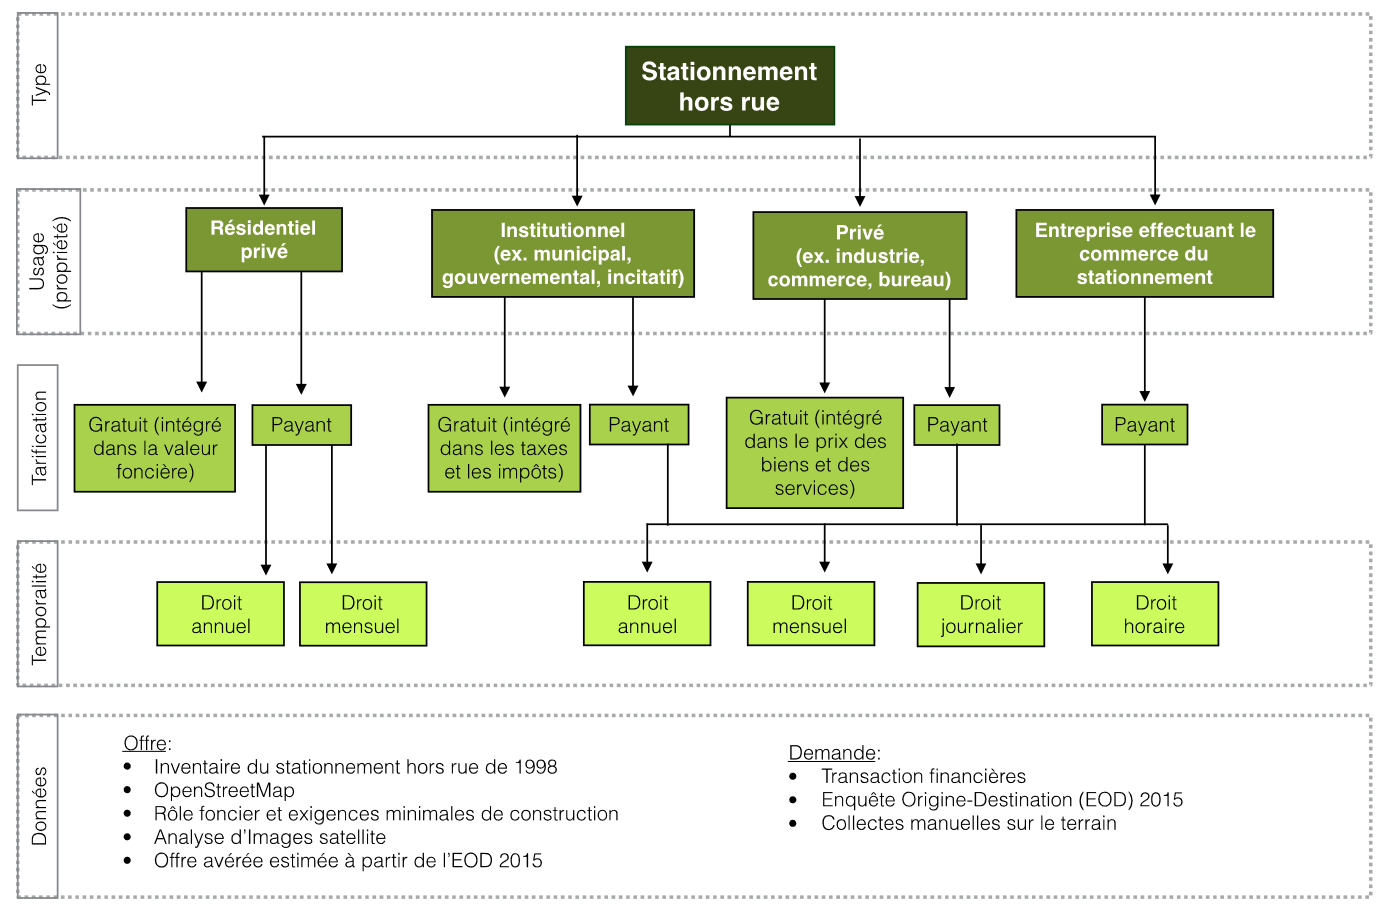
\includegraphics[width=1.0\textwidth]{images/Typologie_Stationnement_hors_rue.png}
    \caption{Typologie de stationnement hors rue. \hl{vérifier droits auteurs} Source: \cite{Morency:StationnementDans:2017}}
    \label{fig:Typo_Stat_hors_rue}
  \end{figure}
\begin{figure}[ht]
    \centering
    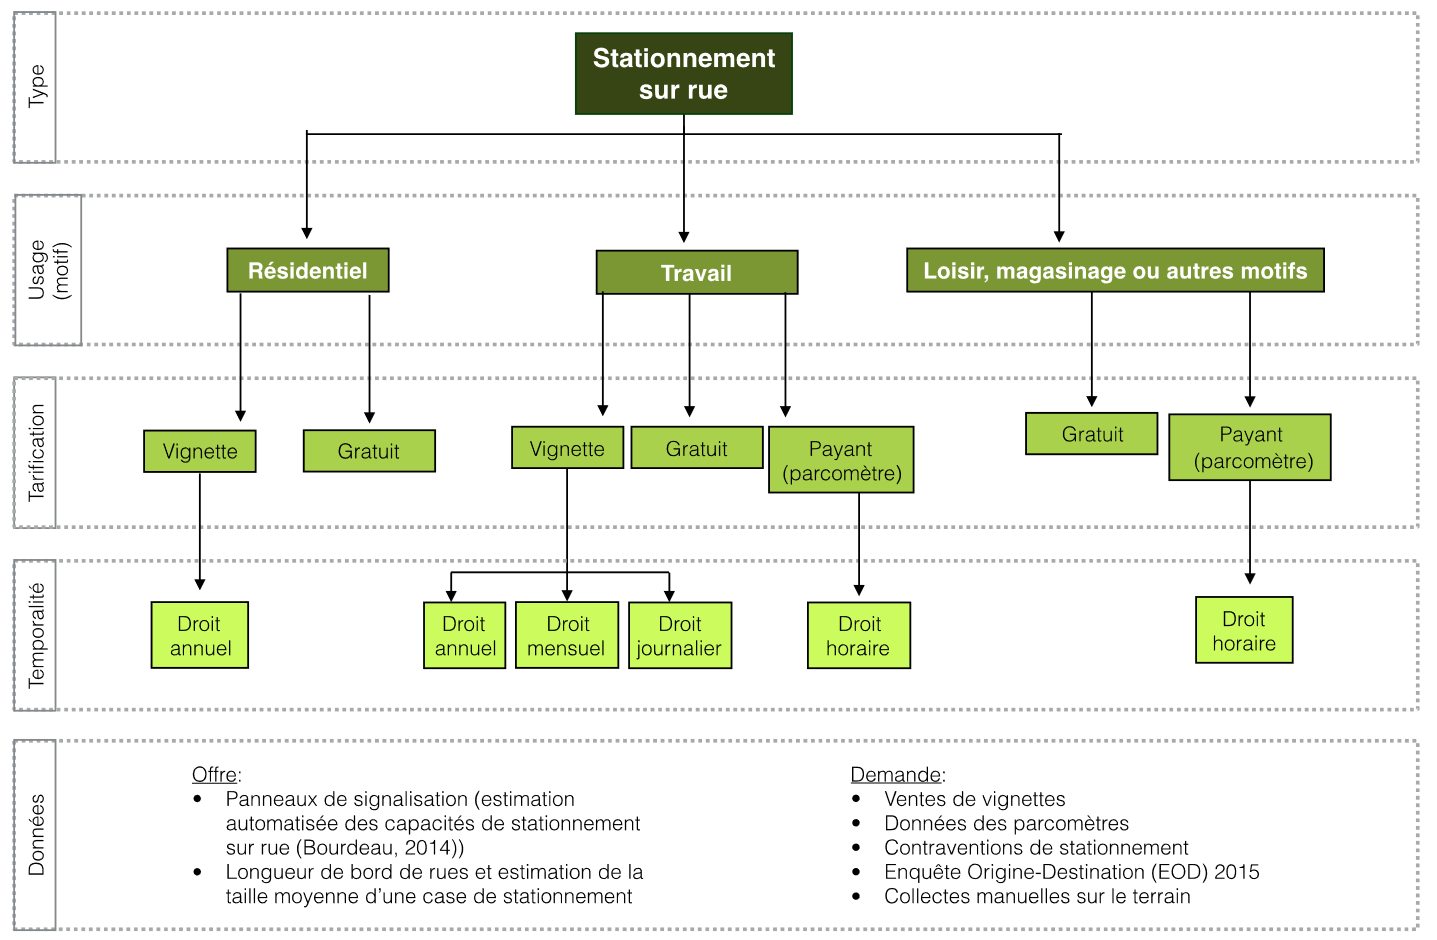
\includegraphics[width=1.0\textwidth]{images/Typologie_Stationnement_sur_rue.png}
    \caption{Typologie de stationnement sur rue. \hl{vérifier droits auteurs} Source: \cite{Morency:StationnementDans:2017}}
    \label{fig:Typo_Stat_sur_rue}
\end{figure}
Il est important de noter qu'il n'existe pas à la connaissance de l'auteur un inventaire tel que celui complété par le ministère des Transports pour la ville de Montréal \parencite{ConsortiumCIMA+-DanielArbouretassocies:InventaireEspaces:1998}.

\section{Méthodes d'inventaire basées sur des données géoréférencées}
La revue de littérature a révélé plusieurs différentes méthodologies utilisées pour recenser l'offre de stationnement hors rue et sur rue. 

\subsection{Hors-Rue}
\textcite{Chester:ParkingInfrastructure:2015} utilisent des données basées sur le rôle foncier, un modèle de croissance de la construction et des données de recensement croisées avec les minimums de stationnement issus des codes d'urbanisme pour inférer la capacité de stationnement de la région de Los Angeles depuis les années '50. Les auteurs indiquent qu'ils estiment que les minimums mis en place sont probablement le nombre de places construites du fait de la valeur marginale basse de la place de stationnement par rapport à la construction de bâtiments. \citeauthor{Chester:InventoryingSan:2022} estime la capacité de stationnement en utilisant une méthode similaire basée sur les codes d'urbanismes et les données foncières pour la région de San Francisco \parencite{Chester:InventoryingSan:2022} et Phoenix \parencite{Hoehne:ValleySundrenched:2019}. \textcite{Scharnhorst:QuantifiedParking:2018} fait pour sa part un inventaire de 5 régions métropolitaines aux États-Unis utilisant encore une fois des méthodes basées sur les codes d'urbanisme en vigueur à la période de construction. Ce dernier n'est cependant pas revu par les pairs. \par 
Il est important de noter que ce type d'inventaire fait l'hypothèse que les promoteurs immobiliers construisent le minimum de places possibles. \textcite{Stangl:ParkingLots:2019} indique que les promoteurs immobiliers ne respectent pas nécessairement cette hypothèse car leur but est de minimiser les risques d'invendus et leurs perceptions ne sont pas alignées avec l'utilisation réelle des stationnements. Ironiquement, les développeurs ont tendance à bâtir plus de stationnements dans des voisinages de typologie \og{Old Urban} \fg{} \parencite{Voulgaris:SynergisticNeighborhood:2017} alors que ce sont précisément les quartiers où les gens ont une plus faible propension à conduire. \textcite{Stangl:ParkingLots:2019} comporte des entrevues avec des promoteurs immobiliers qui illustrent l'effet structurant des minimums de stationnement sur les décisions de construction, mais aussi certains biais dans la prise de décision vis-a-vis du stationnement.

\subsection{Sur-rue}
\textcite{Bourdeau:MethodologieAnalyse:2014} détaille une méthode d'inventaire de places de stationnement sur rue basé sur l'utilisation des données de bords de réseau routiers, de panneaux de stationnement et d'archive cadastrale indiquant les entrées charretières pour déterminer le nombre de places de stationnements sur rue. Cette approche permet de mieux identifier les limites règlementaires et temporelles que les approches utilisées par \textcite{Chester:InventoryingSan:2022} et \textcite{Scharnhorst:QuantifiedParking:2018}. En effet, ces dernières n'enlèvent de la capacité que sur une base de moyennes pour les intersections, arrêts de bus sans prendre en compte la géométrie locale ou des contraintes qui ne peuvent être adéquatement capturées par \ac{OSM}. Dans les 2 cas ci-haut, l'inventaire sur rue est fait avec des largeurs d'intersection moyenne, avec des retraits pour les entrées et la règlementation utilisant des heuristiques plutôt que la réalité du terrain. \par

\section{Méthodes d'inventaire basées sur l'imagerie aérienne}
\textcite{Akbari:AnalyzingLand:2003} utilisent des orthophotos en couleur avec une résolution de 0.3m pour identifier le pourcentage d'utilisation des sols de différentes surfaces (bâtiments, verdure, stationnements, etc.). Une approche de Monte-Carlo est utilisée où un sous-ensemble de pixels se voit assigner une utilisation des sols manuellement pour chaque sous-ensemble de photos basé principalement sur la couleur du pixel. Le nombre de pixels manuellement identifié est validé contre la convergence du pourcentage d'utilisation des sols jusqu'à un seuil de 1\%. Une fois ce sous-ensemble identifié, l'utilisation des sols est assignée à l'ensemble des pixels de l'orthophoto. \citeauthor{Akbari:AnalyzingLand:2003} ne font pas de distinction entre la voirie et le stationnement sur rue.\par
\textcite{Davis:EstimatingParking:2010} recensent un sous ensemble de codes postaux manuellement avant d'utiliser une régression pour estimer le stationnement sur l'ensemble d'un territoire. Une régression basée sur une codification d'\og{urbanité} \fg{} des codes postaux issue du recensement est ensuite utilisée pour inférer l'offre de stationnement hors rue non résidentielle sur un territoire s'étendant sur 4 états dans le Midwest des États-Unis. La méthode est validée sur un sous-ensemble de données qui n'est pas utilisé pour la régression et les auteurs constatent une erreur de 5\% entre la valeur inférée par régression et la valeur mesurée manuellement pour le sous-ensemble de contrôle. Comme l'étude précédente, cette étude n'inclut que le stationnement hors rue. \par
L'augmentation de la capacité de calcul numérique et la démocratisation des méthodes d'apprentissage machine a mené \textcite{Hellekes:ParkingSpace:2023} à utiliser la photographie aérienne et des données \ac{OSM} pour identifier les aires de stationnement à l'aide d'une méthode Dense-U-Net. D'autre part, les auteurs utilisent plusieurs ensembles d'orthophotos d'une même zone et les données \ac{OSM} pour identifier les zones de stationnement non démarquées, intermittentes ou informelles comme les trottoirs et jardins. Des méthodes de régression Bayesienne sont utilisées pour introduire explicitement l'incertitude dans la reconnaissance de l'objet de stationnement. \textcite{Henry:CitywideEstimation:2021} est un autre article par la même équipe de recherche qui donne un aperçu des différentes méthodes d'apprentissage machine utilisées jusqu'à présent pour identifier des objets dans un périmètre urbain. D'autre part, ils indiquent que la méthodologie de fusion choisie influe sur les résultats en fonction du type d'objet reconnu. Par exemple, l'inclusion des données \ac{OSM} améliore l'identification de routes et de voies d'accès, mais nuit à l'identification de stationnement.  \par
\textcite{Yin:ContextenrichedSatellite:2022} est un autre article portant sur l'inventaire de stationnement en utilisant des méthodes d'apprentissage machine pour détecter des stationnements. En plus d'utiliser l'imagerie satellite, les auteurs utilisent des données \ac{OSM} pour ajouter du contexte et voient une amélioration la métrique de de détection \ac{IoU} d'environ 2.5\% en 2 dimensions supplémentaires au tenseur d'images. Les auteurs on en effet pris les couches de bâtiments et de routes d'\ac{OSM} pour donner plus de contexte aux algorithmes d'aprrentissage machines. Les éléments OSM ont généré 15 dimensions supplémentaires au tenseur qui ont été réduit à 3 par convolution et avec une activation en utilisant une fonction tanh. Ce résultat est ensuite additionné au 3 dimensions d'une image RGB. Ils ont par la suite étalloné leur méthode avec plusieurs algorithmes de segmentation d'image: U-Net, U-Net++, LinkNet, D-LinkNet, FPN, PAN, DeepLab v3 et Deeplab v3+. Les algorithmes ont été testés avec et sans contexte et les auteurs constatent que l'algorithme DeepLab v3 performe le mieux particulièrement sur les stationnement de plus petite taille.

\section{Politiques de stationnement}
\subsection{Stationnement hors rue}
Selon \textcite{Shoup:HighCost:2005}, les minimums de stationnement ont vu le jour dans les années 50 en réponse à la croissance du parc automobile et pour assurer que les commerçants et citoyens internalisaient les coûts associés à l'automobile. Ce mécanisme règlementaire est encore omniprésent au Québec puisque seuls les arrondissement de Côte des Neiges, du Sud-Ouest, du Plateau Mont-Royal et du Centre-Ville de Montréal \hl{besoin de citations}. La ville de Québec est en processus d'abroger ces requis pour l'habitation pour les zones en milieu dense ou le long des axes de transport en commun \parencite{VilledeQuebec:AdoptionReglement:2024}.\par
Ces codes ont été utilisés pour faire l'inventaire de stationnement dans plusieurs métropoles. Cela étant dit, l'historique de fusion de municipalités et la difficulté de trouver des codes d'urbanisme avant 1995 rend l'utilisation de ces données relativement difficile. La figure \ref{fig:historique_fusions} montre les fusions successives ayant mené à l'actuelle ville de Québec:
\begin{figure}
  \centering
  \captionsetup{justification=centering,margin=2cm}
  \includegraphics[width = 0.5\textwidth]{images/historique_fusions_VDQ.png}
  \captionsetup{justification=centering,margin=2cm}
  \caption{Diagramme montrant les fusions géopolitiques de la ville de Québec. \hl{Vérifier droits d'auteurs} Source: \cite{VilledeQuebec:ReperesChronologique:}}
  \label{fig:historique_fusions}
\end{figure}


\section{Coûts de provision}
Plusieurs coûts sont associés à la provision de stationnements, autant pour les individus, que pour les collectivités locales ou de tierces parties plus difficiles à identifier dans le cas d'externalités. Cette section visera à identifier quels sont les coûts associés et qui les porte.

\subsection{Propriétaires fonciers et municipalités}
\textcite{Blanc:EffectsUrban:2014} ont estimé la valeur foncière de 6 villes américaines en évaluant la valeur foncière des bâtiments et des stationnements extérieurs. En comparant le tissu urbain entre 1950 et 2010, les auteurs ont estimé la différence de valeur foncière et de revenu entre les deux configurations. Dans certains, les municipalités avaient accepté de détruire leur centre-ville pour permettre le développement de tours à bureaux entourées de stationnements. Dans d'autres, les municipalités avaient largement conservé le tissu urbain d'avant guerre. Dans tous les cas, le revenu foncier associé au stationnement était entre 5 et 10x moindre que le revenu associé aux bâtiments. L'étude est cependant associative puisqu'il est difficile d'isoler la nature causale entre la dilution du revenu foncier et la provision de stationnements, mais illustre les coûts d'opportunité associés à l'entreposage de véhicules personnels. \par

\section{Effet de l'offre de stationnement sur la mobilité}
\textcite{Chester:ParkingInfrastructure:2015} constatent que la capacité de stationnement est la plus haute dans le centre de la ville, mais que la croissance du parc de stationnement a principalement lieu sur le périmètre de la région.  Ils constatent aussi que le parc de stationnement a cru plus vite que la capacité routière, mais a suivi l'offre de stationnement résidentielle.\par
\textcite{Guo:DoesResidential:2013} créé un modèle logit imbriqué pour identifier l'effet de l'offre de stationnement sur la motorisation des ménages de l'enquête OD de New York et trouve que la disponibilité de stationnement dans l'entrée et en bord de rue est potentiellement un plus grand déterminant de la motorisation qu'un garage. L'auteur suggère aussi que les programmes de vignette ont potentiellement des conséquences inattendues où la réduction de l'achalandage des stationnements par les non-résidents mène à une motorisation accrue des résidents, éliminant l'effet bénéfique de la réduction de l'offre des non-résidents. D'autre part, l'auteur trouve que la présence de nettoyage de rue réduit l'utilité marginale d'un véhicule supplémentaire et réduit la motorisation. Ces constats sont cependant limités au contexte de New York qui est une ville relativement dense avec une bonne desserte de transport en commun.\par
\textcite{Yin:BuiltEnvironment:2018a} associent eux aussi de manière significative la disponibilité du stationnement aux deux extrémités des déplacements à la possession et l'utilisation accrue d'automobile quoique la formulation des résultats rend difficile l'interprétation de la taille de l'effet.\par
\textcite{Weinberger:ResidentialOffStreet:2009} font une analyse comparative entre Jackson Heights et Park Slope à New York. Jackson Heights a une part modale en auto-solo vers le centre-ville qui ne suit pas les principaux indicateurs de la motorisation (le revenu du ménage et la densité) et qui n'est pas expliqué par la desserte en \ac{TC} des deux quartiers. Les auteurs estiment l'offre de stationnement au travers du registre \ac{PLUTO} pour les bâtiments de 4 logements et plus ainsi qu'un échantillonnage pour les bâtiments comportant moins de 4 logements. Les auteurs ont constaté que Jackson Heights a 156\% plus d'offre de stationnement. Malgré le fait que Park Slope ait 46\% plus de stationnements en structure et en surface hors résidence, Jackson Heights a quatre fois plus d'espaces de stationnements privatifs dans les résidences. Les auteurs établissent ensuite des prospectives pour le développement résidentiel planifié par la ville et estiment que les résidents de ces nouveaux développements auront entre 42 et 49\% plus de chance d'être motorisés que les habitants actuels du fait des requis de stationnements minimums actuellement en effet. Bien que l'étude ne soit pas très robuste statistiquement, les auteurs concluent que les requis de stationnement minimum ne sont pas une bonne politique puisqu'ils effritent la qualité de l'environnement pour les marcheurs et augmentent l'attractivité de la possession d'une automobile. Les auteurs encouragent une étude systématique des liens entre la provision de stationnements, la motorisation et le choix modal.\par
Deux études dans le contexte norvégien \parencite{Christiansen:ParkingFacilities:2017,Christiansen:HouseholdParking:2017} créent des modèles associatifs à partir d'enquêtes origine destination nationales. \textcite{Christiansen:ParkingFacilities:2017} trouvent que la limitation de la capacité de stationnement au travail avec une tarification est le moyen le plus efficace pour réduire la part modale de l'automobile pour ce type de trajet. Une tarification horaire ou journalière est aussi plus efficace pour réduire les trajets automobiles puisque le coût marginal pour chaque utilisation du stationnement est perçu par l'utilisateur. D'autre part, les auteurs trouvent que la proximité du stationnement au lieu d'habitation dans les milieux denses avec beaucoup d'offres de service à proximité. Les auteurs indiquent cependant qu'il y a des risques d'autosélection et d'endogénéité avec leur étude, un problème récurrent avec les études reliées au stationnement \parencite{Inci:ReviewEconomics:2015}. \textcite{Christiansen:HouseholdParking:2017} comparent les comportements de mobilité pour différents degrés d'accès au stationnement à la résidence. Ils trouvent qu'une distance d'accès supérieure à 50m a un effet marqué sur le choix modal sans affecter le nombre de trajets. Les trajets non contraints voient une plus grande différence de choix modal que les trajets motif travail. D'autre part, ils constatent peu de différence dans les taux de mobilité entre les ménages motorisés et non-motorisés, inférant que les dispositions de stationnement et de motorisation ont peu d'effet sur le bien-être. Les auteurs concluent qu'une gestion intégrée du stationnement qui inclut une combinaison d'une tarification 24/7 de règlements qui séparent le stationnement du logement physiquement et juridiquement et une gestion du nombre total de places de stationnement sont des leviers utiles pour gérer la demande de transport. Ils constatent le manque de lien causal dans leur étude, qui bien que non nécessaire pour l'établissement de politique efficace, est regrettable d'un point de vue scientifique.\par 
Dans le contexte chinois, \textcite{Yin:BuiltEnvironment:2018a} dressent des constats similaires à \textcite{Christiansen:HouseholdParking:2017} et \textcite{Christiansen:ParkingFacilities:2017} quant à l'influence de la disponibilité du stationnement à l'origine et la destination d'un trajet, même en contrôlant pour l'utilisation du territoire et les variables sociodémographiques, mais utilisent seulement des mesures agrégées de disponibilité totale de stationnement.\par
\textcite{Currans:HouseholdsConstrained:2023} crée un modèle de régression et une analyse de médiation pour lier l'effet de l'offre de stationnement résidentiel hors rue avec la motorisation et les kilomètres parcourus par ménage et constatent que les ménages ayant des contraintes de stationnement (moins d'un stationnement par unité) parcourent moins de 10-23\% moins de kilomètres à typologie de voisinage constante. Les auteurs encouragent la présence de plus de questions sur les conditions de stationnement dans les enquêtes ainsi qu'à la création d'un inventaire de stationnement. \par
\textcite{McCahill:EffectsParking:2016} observe la relation entre la provision de stationnements avec la part modale de l'automobile sous le prisme du critère de Bradford-Hill pour inférer que la provision de stationnements est la cause probable de l'augmentation de la part modale de l'automobile. \hl{cet article est intéressant mais le critère est très sujet à interprétation}

\section{Allocation, tarification et ratissage}
Une littérature économique riche existe sur les différents mécanismes d'allocation de places de stationnement qui est résumée par \textcite{Inci:ReviewEconomics:2015}, sur laquelle est largement basée cette section. Dès les premiers pas de la discipline, dans les années 50, la mise en place d'une tarification sur les infrastructures routières, variable dans le temps et l'espace, est identifiée comme une condition nécessaire pour réduire les externalités reliées au ratissage, la congestion et les externalités liées au transport urbain de personnes \parencite{Vickrey:StatementJoint:1994}. Les tentatives les plus intéressantes d'instaurer un marché variable viennent de San Francisco et Seattle où des projets pilotes ont été implémentés. Les études portant sur ces deux pilotes ont trouvé que la demande est initiallement inélastique, mais que le maintien de la politique amène des améliorations sur la disponibilité à long terme. \textcite{Chatman:TheoryImplementation:2014} constatent que l'implémentation de SFPark, le programme de tarification variable de San Francisco, ont eu des résultats mitigés. Bien que le taux d'occupation moyen, qui était l'indicateur utilisé pour faire varier la tarification,  ait été réduit à environ 80\%, le taux de disponibilité (le pourcentage de temps où au moins une place est disponible sur un tronçon) n'était pas sensible au prix avec les modalités politiques, l'imposition de prix plafond, la lenteur de l'adaptation du prix et le choix d'indicateur pour la tarification sont déterminants pour réduire les externalités liées à la recherche de stationnement. Cela amène un questionnement plus large sur la viabilité politique d'un système de tarification.\par
\textcite{vanOmmeren:RealPrice:2011} infèrent la propension à payer pour un stationnement des résidents d'Amsterdam en utilisant les préférences révélées par le choix d'achat de résidence. En utilisant des données de ventes de résidences et en capitalisant la différence de prix sur le temps d'attente pour un permis de stationnement résident, les auteurs estiment une propension à payer de 10€ par jour, bien au-dessus du prix réel de 0.40€ et bien en dessous des recettes possibles pour les places tarifées aux visiteurs qui paient 2.3€ par heure.\par
\textcite{Inci:ReviewEconomics:2015} mentionne les éléments suivants comme manquants à la recherche: l'effet de la prévention de la fraude, l'économie politique du stationnement, les interactions entre véhicules stationnés et en mouvement et l'établissement de l'élasticité de la demande dans plusieurs contextes spacio-temporels. Il est intéressant de noter qu'aucune mention n'est fait des coûts d'opportunités infligés aux autres modes ou activités par le stationnement dans la revue économique.

\section{Utilisation de la capacité existante}
\textcite{Translink:2018Regional:2019} a sondé les taux d'occupation des blocs-appartements et du stationnement sur rue dans la grande région de Vancouver. Pour l'échantillon donné, entre 30 et 40\% de la capacité de stationnement n'était pas utilisée. L'étude constate aussi que la demande de stationnement est plus faible chez les locataires que les propriétaires. Cela étant dit, l'étude ne recale pas les résultats sur l'ensemble du parc immobilier et n'utilise pas de test statistique pour valider la significativité de leurs résultats. La conception de l'étude n'a pas permis de quantifier les interactions entre le stationnement hors rue et sur rue pour les blocs appartements, mais indique qu'anecdotiquement, les praticiens ont constaté que les résidents utilisaient le stationnement sur rue plutôt qu'en sous-sol lorqu'il n'y avait pas de restriction sur le stationnement sur rue. 

\section{Stationnement et utilisation du territoire}
\textcite{Chester:ParkingInfrastructure:2015} trouvent que 16\% de la région est utilisée pour le stationnement, plus que l'ensemble du réseau routier. D'autre part, le centre-ville a vu une forte croissance de stationnements en structure et sous-terrains où les valeurs de terrains sont hautes. Les auteurs concluent qu'il y a 3.3 places de stationnement par véhicule et que la majorité de la croissance du parc de stationnement a eu lieu entre 1950 et 1980.\par

\textcite{Davis:EstimatingParking:2010} estiment que 4.97\% de l'espace urbain est utilisé par le stationnement hors rue commerciale (sans compter les stationnements sur rue ou résidentiels). Ils estiment environ 1.8 places par voiture, 5.3 places par ménage et 1.7 places par adultes. À noter que l'indicateur ne mesure pas la même chose que \textcite{Chester:ParkingInfrastructure:2015} puisque ce dernier inclut les stationnements sur rue et résidentiel.

\section{Reconnaissance d'images}
Les problèmes de reconnaissance d'images se divisent en trois types de solution; la classification consiste à dire si une image contient un objet ou appartient à une classe d'image; la détection consiste à trouver un objet dans une image et à l'illustrer typiquement au moyen d'une boîte englobante; la segmentation sert à illustrer les contours détaillés d'un objet, les classifications se font typiquement pixel par pixel selon différentes classes. Les méthodes de segmentation d'instance sont un hybride des méthodes de détection et de segmentation. Dans ces problèmes, des instances de chaque type sont identifiées au moyen de boites englobantes puis un masque est généré pour le type pour illustrer l'objet. La figure \ref{fig:computer_vision_problems} représente le résultat de différents processus d'apprentissages sur une même image:

\begin{figure}
  \centering
  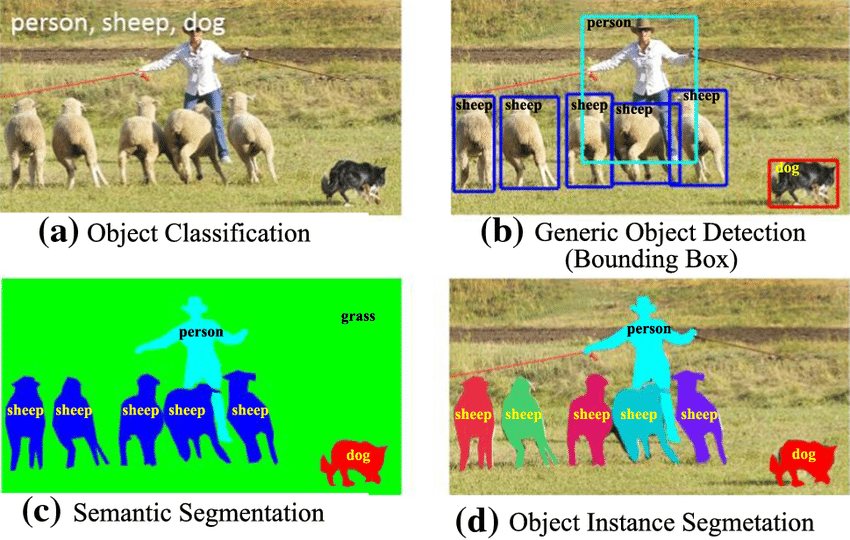
\includegraphics[width = 0.5\textwidth]{Recognition-problems-related-to-generic-object-detection-a-image-level-object.png}
  \caption{Résultat de différentes méthodes de vision par ordinateur pour une même image.\hl{vérifier droits d'auteurs} Source: \cite{Minaee:ImageSegmentation:2022}}
  \label{fig:computer_vision_problems}
\end{figure}
Les processus varient aussi dans leur résultante. Tandis que les modèles de segementation pure feront une affectation de la même couleur à plusieurs objets d'un même type, la segmentation d'instance rend le processus de post traitement des raster plus simple en donnant une couleur différente à chaque instance d'un même type d'objet. Cette dernière propriété a le mérite de potentiellement faciliter le post traitement des résults.
\FloatBarrier
\subsection{Algorithmes de détection}

\subsection{Algorithmes de segmentation}

\subsection{Algorithmes de segmentation d'instance}
La première est la segmentation sémantique qui consiste à séparer des pixels dans une image par classe. La deuxième est la segmentation d'instance. Cette dernière reconnait des objets, le classifie et en extraie le contour. \textcite{He:MaskRCNN:2018} est l'article original sur la méthode qui a par la suite été adapté dans un contexte de reconnaissance SIG \parencite{Pesek:MaskRCNN:2018} ou pour la reconnaissance automatique de terrains sportifs pour réinjecter les polygones directement dans \ac{OSM} \parencite{Remillard:JremillardImagestoosm:2024}.\par
\textcite{Fritz:InstanceSegmentation:2020} développe plusieurs estimés de segmentation d'instance pour des bâtiments à l'aide de deux modèles. Le premier est celui cité plus haut\parencite{He:MaskRCNN:2018} tandis que le deuxième est un modèle de segmentation d'image modifié pour segmenter les instances \parencite{Iglovikov:TernausNetV2Fully:2018} une fois la segementation d'image complétée

\subsection{Bases de données disponibles}
Deux enjeux sont critiques au succès d'un projet d'apprentissage machine. La présence d'un modèle adapté à la tâche en cours et la présence d'un jeu de donnée annoté qui peut être utilisé pour ajuster les poids initiaux du modèle pour permettre de modifier les poids du modèle et permettre de l'appliquer à de grands ensembles de données. Le tableau suivant résumera les jeux de données actuellement disponibles pour la segmentation sémantique en milieu urbain:
\begin{table}
 \centering
    \begin{tabular}{l p{0.2\textwidth} l p{0.3\textwidth}  p{0.2\textwidth} l} 
    \hline
    Nom & Origine & $N_{classes}$ & Classes pertinentes au stationnement & Point de vue\\
    \hline
    CNRParkEXT & \cite{Amato:DeepLearning:2017} & 2 & Places occupées, places libres & Caméra de surveillance \\
    PKLot & \cite{deAlmeida:PKLotRobust:2015} & 2 & Places occupées, places libres & Caméra de surveillance \\
    APKLot & \cite{Hurst-Tarrab:RobustParking:2020} & 1 & Grappes & Imagerie satellite\\
    Skyscapes & \cite{Azimi:SkyScapesFineGrained:2019} & 31 & Aires pavées, aires non-pavées & Orthophotos\\
    Grab-PkLot & \cite{Yin:ContextenrichedSatellite:2022} & 1 & Aires de stationnement & Orthophotos\\
    \hline
   \end{tabular}
   \caption{Jeux de données annotés de segmentation sémantique en milieu urbain}
   \label{tab:jeux_donnees_segmentation_urbain}
\end{table}